%!TEX TS-program = pdflatexmk

% Copyright (c) 2018 - 2022, Martin Scheidt (ISC license)
% Permission to use, copy, modify, and/or distribute this file for any purpose with or without fee is hereby granted, provided that the above copyright notice and this permission notice appear in all copies.

\documentclass[border=2]{standalone}

\usepackage[dev]{tikz-trackschematic}

\begin{document}
  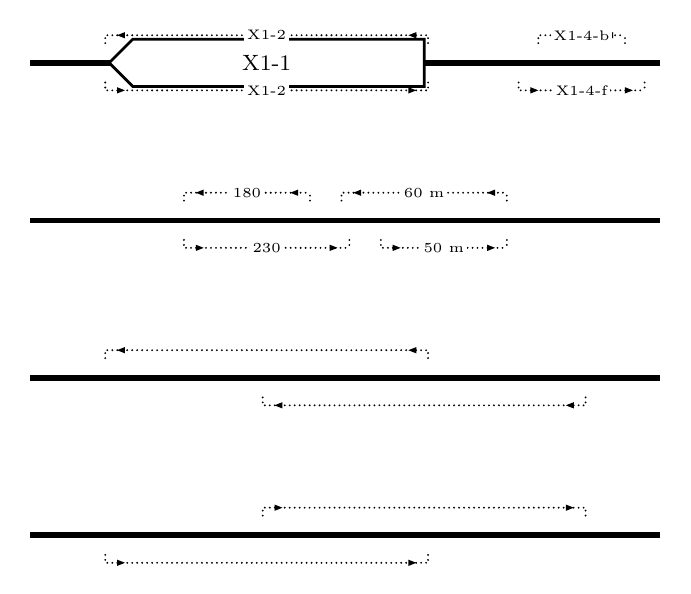
\begin{tikzpicture}
  
    \foreach \i in {1,2,...,4}{% base coordinate
      \coordinate (A\i) at ($(0,0) + 2*(0,-\i)$);% base coordinate
      \coordinate (B\i) at ($(8,0) + 2*(0,-\i)$);% base coordinate
    }

    \foreach \i in {1,2,...,4}{% draw main tracks on base coordinate
      \maintrack (A\i) --   (B\i);
    }

    \foreach \i in {1,2,...,4}{% coordinates for testing symbols
      \coordinate (X\i-1) at ($(1,0) + 2*(0,-\i)$);
      \coordinate (X\i-2) at ($(3,0) + 2*(0,-\i)$);
      \coordinate (X\i-3) at ($(5,0) + 2*(0,-\i)$);
      \coordinate (X\i-4) at ($(7,0) + 2*(0,-\i)$);
    }

    \train[backward] at (X1-1) label (X1-1);

    \berth[bidirectional]  at (X1-2) length (X1-2);
    \berth[forward,length=1.5cm] at (X1-4) length (X1-4-f);
    \berth[backward,length=1cm]  at (X1-4) length (X1-4-b);

    \berth[forward,length=2cm]    at                   (X2-2) length (230);
    \berth[backward,length=1.5cm] at ([shift={(-0.25,0)}] X2-2) length (180);
    \berth[forward,length=1.5cm]  at ([shift={( 0.25,0)}] X2-3) length (50~m);
    \berth[backward,length=2cm]   at                   (X2-3) length (60~m);

    \berth[backward] at (X3-2) length ();
    \berth[position=left,backward] at (X3-3) length ();
    \berth[forward]  at (X4-2) length ();
    \berth[position=left,forward]  at (X4-3) length ();

  \end{tikzpicture}
\end{document}